\chapter{Implementation}

As we repeatedly mentioned in the first chapter, the design we chose should allow multiple implementations for each module. The implementations provided in this thesis are designed for use-cases ranging from beginner user that requires only core functionality to advanced users who can utilize full module distribution. The resulting implementation therefore offers a monolithic application as well as separate modules.
\par
In this chapter we will discuss the implementation details of every module. At the beginning we will explain our programming language choices. We will add a short description for every library that we used and a reason why we preferred it to others.

%%-----------------------------------------------------------------------------------------
%% SECTION
%%-----------------------------------------------------------------------------------------
\section{Programming Language}

First decision we had to take was to select a suitable programming language. We had to follow the main guidelines that we have set earlier. That is, we had to find a way to support multiple platforms, while in the same time we needed flexible enough language to handle our modular design and fast enough to help us with scalability.
\par
Even though our modules are separable and therefore each of them could be written in a different language, we wanted to reduce the amount of used languages to minimum, ideally just one or two for the sake of simplicity. Furthermore, we focused on languages that would allow us to write one implementation for all platforms with the minimum of tweaks. Last but not least, we wanted a language that we had at least some experience with.
\par
We have narrowed the choice to three possible main programming languages for our implementation: C++, C\# and Java. All of them are major languages, have cross-platform capabilities and are well-established with enough libraries for all our features. We excluded popular languages Python and JavaScript due to their nature as scripting languages and therefore not providing enough performance for a bigger scale project.

%%-----------------------------------------------------------------------------------------
\subsection{GUI struggles}

The weak spot of all three languages is graphical user interface~(GUI) necessary for our Manager module. We would like the module to be modern and visually attractive and common GUI frameworks are usually either platform-specific, difficult to work with or have too many limitations. The exception might be
Qt~\citep{qt}, which is a very capable GUI toolkit written in C/C++, plus there is a Java wrapper for this library available.
\par
In the past few years, web applications have become very popular. Increasing performance of personal computers and development in web technologies as well as rise of single-page application frameworks allowed the creation of applications running almost entirely in a web browser. Nowadays, many people use only web browser on their computer where they have access to all sorts of web applications for any purpose. This has also changed their perception of how user interface should look like. Following this trend there are some desktop applications written entirely using web technologies, enclosed in a web browser wrapper.
\par
We decided to adopt above-mentioned approach for our Manager module. There is an open-source project written in C++ called Chromium Embedded Framework~(CEF). CEF focuses on facilitating embedded browser use cases in third-party applications~\citep{cef}. It means that we can create GUI using HTML5 and JavaScript relying on flexibility, cross-platform support and relative simplicity that they provide compared to other options. CEF offers a way to call C++ code from JavaScript so we can further customize its behavior as a proper desktop application.
\par
It is important to note that this decision was influenced by the desire to provide both modular as well as monolithic-looking application. Web GUI can be written once and then be utilized as a stand-alone module running on any web browser or wrapped as desktop application using CEF. Moreover, we can extend it using C++ to bundle it up with the remaining modules and create all-in-one application. Finally, it integrates well with our Database module as Firebase provides its SDK in JavaScript.

%%-----------------------------------------------------------------------------------------
\subsection{Final decision}

Having chosen a programming language and additionally a framework for Manager module, it remains to choose it for Player and Fileserver modules. Out of the three preselected languages we made C++ our final decision.
Both other languages would be equally capable for the task, but C++ provides more performance and more control of memory management. Furthermore, it does not rely on a virtual machine and is already utilized within our Manager module. Lastly, these two modules contain a lot of low-level programming, what makes C++ a preferable candidate and a lot of related libraries are written directly in C/C++.

%%-----------------------------------------------------------------------------------------
%% SECTION
%%-----------------------------------------------------------------------------------------
\section{Fileserver Module}

This module consists of two main parts - file storage and RESTful interface. We used SQL database to store music file metadata and its location in file system and playlists. The REST API follows predefined interface. It adds additional resources for file management as its selected way to manage content.

\subsection{Libraries Used}
We used two third-party libraries for the implementation of this module.
\par
First one is SQLite that we used for data storage. SQLite is a C-language library that implements a small, fast, self-contained, high-reliability, full-featured, SQL database engine. SQLite is the most used database engine in the world. SQLite is built into all mobile phones and most computers and comes bundled inside countless other applications that people use every day. The SQLite file format is stable, cross-platform, and backwards compatible and the developers pledge to keep it that way through at least the year 2050. SQLite database files are commonly used as containers to transfer rich content between systems and as a long-term archival format for data. There are over 1 trillion SQLite databases in active use~\citep{sqlite}. It allows us to to create a small SQL database file locally on the device where it runs.
\par
The other library we used is called C++ REST SDK~(cpprestsdk). The C++ REST SDK is a Microsoft project for cloud-based client-server communication in native code using a modern asynchronous C++ API design. This project aims to help C++ developers connect to and interact with services. Microsoft have developed this library, because historically C++ developers have been lacking a basic set of tools that enable them to access and author REST services in a productive, scalable and asynchronous manner. C++ Rest SDK aims to alleviate some of the pain felt by developers by providing a cross-platform library that is modeled on simplicity, extensibility and composition~\citep{cpprestsdk}. Even though C++ is not a preferred language for creating REST services, this library offers a simple way for both creating and accessing these services. It handles the network communication for us and allows us to focus on the business logic that processes and delivers data.
\todo{maybe add that their are open source and cross platform? mention troubles with cpprestsdk?}

%%-----------------------------------------------------------------------------------------
\subsection{Data Storage}
Usually, all song files contain metadata besides the actual music data. They contain information such as song title, author, album, or genre and are stored in a data structure called tag. Reading it from the file repeatedly is hugely ineffective so we read them only once when the file is added to the library. After that, we need to store it somewhere along with the path to the file, as they may be scattered across the file system.
\par
There are multiple possibilities of how to store it. The API requires the ability to search in the library so the common approach would be to store the data in a relational database. This implementation is intended to support a single or up to just a couple of users - its purpose is to allow users to create their own music library. Therefore, utilizing a dedicated database server is unreasonable. Instead, we used SQLite library as it provides a full-featured SQL database engine in a single library. It can easily store thousands of records which is sufficient.

%%-----------------------------------------------------------------------------------------
\subsubsection{Code Remarks}
In the code, we created a single class that takes care of working with the database. We named it \texttt{SqliteAPI}, as it provides an API for working with our SQLite library. This class handles SQL query creation and communication with database. Since all its methods are called from REST API calls, they all return an error code so in case an error occurred it can be reported to caller. The actual return value is then passed in a form of out parameter. Methods that retrieve data accept a list of parameters that allow filtering and modifying the results of their query.
\par
Additionally, this class contains functionality for adding new music files to library. It utilizes tinyfiledialogs library to display cross-platform file dialogs to allow users to choose new files. To extract metadata from these files we used ffmpeg library. We will talk further about this library in the Player Module section \todo{forward referencia, skusit vymysliet inak} where we utilize it for decoding. Here, we used its capability to read music files and retrieve metadata which are then stored in the database. This functionality is wrapped in \texttt{AudioInspector} class.

%%-----------------------------------------------------------------------------------------
\subsubsection{Database Schema}
\begin{figure}[ht]\centering
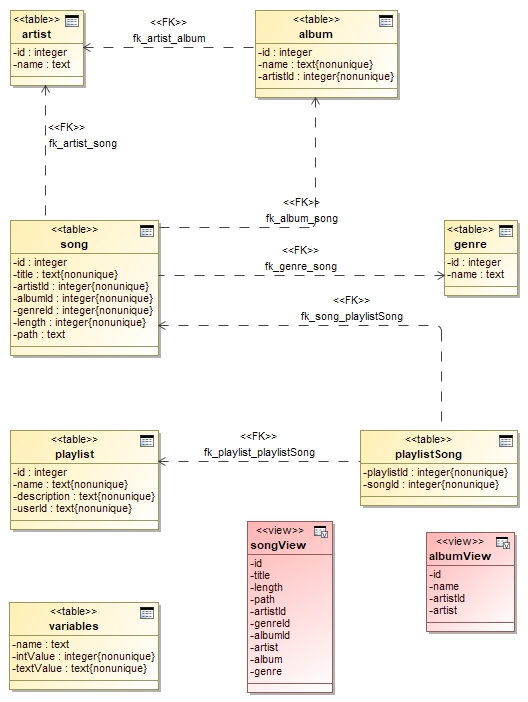
\includegraphics[width=1.0\textwidth]{img/DbDiagram2.png}
\caption{Database schema}
\label{fig03:dbSchema}
\end{figure}

%%-----------------------------------------------------------------------------------------
\subsection{Rest API}
Creating a REST API in C++ was not an easy task. There are many more suitable programming languages for that. However, C++ REST SDK library provides a lot of tools to make it easier than integrating with an API written in a different language. It provides a HTTP listener that listens for incoming requests and a set of asynchronous methods to handle these requests in a modern and effective way. For this, it provides its own implementation of asynchronous tasks.

%%-----------------------------------------------------------------------------------------
\subsubsection{Code Remarks}
To create an abstraction between the HTTP listener and data storage we utilized the bridge design pattern. It allowed us to create HTTP listener independent from data storage. Coupling it with another data storage would just require implementing the abstract class \texttt{AbstractFileServerHandler} in a new bridge.
\par
The \texttt{FileServerAPI} class is the implementation of the mentioned listener. It listens for HTTP requests on chosen address and port. It supports \texttt{GET}, \texttt{POST}, \texttt{PUT} and \texttt{DELETE} request methods required by Fileserver API design and adds \texttt{OPTIONS} method to provide cross-origin resource sharing~(CORS) headers. These are important to allow Manager module running on a browser that restricts cross-origin HTTP requests to access this API. Upon receiving a request a corresponding method handler parses and verifies the URI and parameters to determine the resource. Then it passes the parameters to a correct method of the associated bridge which executes the action and returns payload for the response. This response is then sent back to the client.
\par
\texttt{FileServerHandler} class is the bridge implementation for SQLite data storage. This bridge is the owner of \texttt{SqliteAPI} instance and translates REST API calls to \texttt{SqliteAPI} calls and translates data returned by \texttt{SqliteAPI} to JSON format supported by REST API.

%%-----------------------------------------------------------------------------------------
%% SECTION
%%-----------------------------------------------------------------------------------------
\section{Player Module}

The main feature of Player module is playing music. Besides that, it is important to have music files ready for playback as they might not be stored on the same device. We implemented simple but reliable caching functionality to provide us with reliable amount of the files on demand. Lastly, we implemented a required WebSocket-based communication interface.

%%-----------------------------------------------------------------------------------------
\subsection{Libraries Used}
We utilized three third-party libraries in this module. Two are used for audio playback and one for communication interface.
\par
FFmpeg is the leading multimedia framework, able to decode, encode, transcode, mux, demux, stream, filter and play pretty much anything that humans and machines have created. It supports the most obscure ancient formats up to the cutting edge. No matter if they were designed by some standards committee, the community or a corporation. It is also highly portable: FFmpeg compiles, runs, and passes testing infrastructure FATE across Linux, Mac OS X, Microsoft Windows, the BSDs, Solaris, etc. under a wide variety of build environments, machine architectures, and configurations~\citep{ffmpeg}. Basically, this library allows us to support any music file format we  would like to. We utilised it in Fileserver module for metadata extraction, but it is utilised more heavily here for audio decoding.
\par
To output decoded audio to speakers, we used PortAudio library. PortAudio is a free, cross-platform, open-source, audio I/O library. It lets you write simple audio programs in 'C' or C++ that will compile and run on many platforms including Windows, Macintosh OS X, and Unix (OSS/ALSA). It is intended to promote the exchange of audio software between developers on different platforms. Many applications use PortAudio for Audio I/O~\citep{portaudio}. This library offers cross-platform access to audio I/O as all platforms have their own way of working with it.
\par
Even though C++ REST SDK that we used in Fileserver module promises WebSocket functionality, it only supported WebSocket client at the time. We need to build a WebSocket server so we had to choose different library. For this task we chose Boost.Beast library. Beast is a C++ header-only library serving as a foundation for writing interoperable networking libraries by providing low-level HTTP/1, WebSocket, and networking protocol vocabulary types and algorithms using the consistent asynchronous model of Boost.Asio~\citep{beast}. While this library provides low-level tools, we needed to build just a small server so it allowed us to customize it to create simple and small implementation with the benefits of asynchronous programming from Boost.Asio library.
\todo{write about boost, ffmpeg and portaudio}

%%-----------------------------------------------------------------------------------------
\subsection{File Caching}

The requirements for file caching from analysis are to support two queues and to have a full song ready for playback while another finishes. The second one is important to provide smooth playback without pauses for buffering. We had two options where to store the cached songs - in memory or on hard drive. We decided to store it in memory.
\par
The hard drive option would allow us to cache more songs. That would allow the application to work better on places with slower or less stable internet connection. On the other hand, it is much slower first to store the data and then to decode it, just to delete it afterwards. Additionally, SSD drives and flash memories that are becoming more popular recently do not handle such frequent writes very well and frequent usage of our application would wear these drives down too early.
\par
Storing cached music files in memory reduces the amount of data transfers and files are instantly ready for decoding. However, we can not store too many files as miniature PCs, that might be utilised by this module, do not have too much memory space to spare. Therefore we cache only two files at once in each queue plus one that is being played, 5 in total. When a song is dequeued for playback a new one gets cached, so by the time it finishes there are two songs prepared again. With estimated average size of a music file using compressed file format to be 10MB, we would require around 50MB for our cache. That should not create any problems. Even using lossless file formats where file sizes are around 70MB we would need only 350MB - a machine with 1GB RAM space should handle this module easily.
\par
This solution is volatile to frequent skipping of songs as big music files take time to get cached. However, this application is intended to provide continuous music playback without supervision and skipping songs should be used just as a tool to deal with malicious behavior such as ordering same song multiple times.

%%-----------------------------------------------------------------------------------------
\subsubsection{Code Remarks}

Cache is represented by \texttt{SongCache} class. This class implements all logic required for caching songs. It contains HTTP client from C++ REST SDK library that it uses to download music files to cache. Furthermore, it implements the algorithm for choosing the next song defined in first chapter. It provides two inputs for song queues and outputs next song to be played. Cache is bound to a certain Fileserver module defined upon its creation. It can be reset to clear its contents, but to bind to a new Fileserver, one needs to create a new instance.
\par
Internally, \texttt{SongCache} utilizes \texttt{SongCacheItem} class for storing each queued item. This class holds an asynchronous buffer that is used to download the data asynchronously and upon completion it provides a \texttt{std::basic\_istream} for reading cached file contents. Before accessing it, it is necessary to check for errors.

%%-----------------------------------------------------------------------------------------
\subsection{Communication Protocol}

This module should support communication channel over WebSocket to communicate with Manager module. Player module has the role of server that listens and awaits connection from a Manager module. For that purpose we implemented a simple server that listens for incoming connections. Upon receiving a WebSocket handshake, a session is started and the server stops listening for more connection attempts until the session ends. Within a session, Manager and Player module exchange RPC messages encoded in JSON. The incoming message is checked for validity and then processed. Extracted parameters, if any, are passed to the correlating method, which is then invoked. If it needs to send one or more messages back, they are buffered and sent after the method finishes. To provide some defense against abuse there is a mechanism that ends the session after three consecutive invalid messages. 

%%-----------------------------------------------------------------------------------------
\subsubsection{Code Remarks}

The functionality of the server is layered into multiple classes. At the top is the \texttt{API} class. This class wraps the entire server and technically also the entire module functionality, as whole module is controlled directly through this communication protocol. It offers methods to start and stop the server.
\par
When the server is started, \texttt{API} class instance runs an instance of \texttt{Listener} class. This class provides functionality to listen for and accept incoming connections asynchronously.
\par
After a new connection is accepted, an instance of \texttt{Session} class takes over the created socket and handles the incoming ant outgoing communication. It represents a session of Player module during which the music playback occurs. This instance owns song cache and music player and takes care of cooperation between them. Reads and writes on WebSocket are performed asynchronously. 

%%-----------------------------------------------------------------------------------------
\subsection{Audio Decoding and Playback}

For audio decoding and playback we utilize two libraries - ffmpeg and PortAudio. PortAudio supports asynchronous playback by providing a callback function which is run every time audio device needs more data to output. Within this callback we run a function that decodes required amount of samples using ffmpeg library and writes it to output buffer. This loop runs until we reach the end of music file or the playback is paused.

%%-----------------------------------------------------------------------------------------
\subsubsection{Code Remarks}

Most of the music player functionality is contained within \texttt{MusicPlayer} class. Besides that there are two global static callback functions that are required by PortAudio and two global functions required by ffmpeg. By default, ffmpeg library supports decoding from file. To support decoding from \texttt{std::basic\_istream} utilized by song cache we had to provide custom read and seek functions. PortAudio callback function provides a pointer to a data structure of choice to keep context as this function is global. We use \texttt{StreamInfo} structure. It holds both PortAudio and ffmpeg data members as well as additional information about the state of the playback.
\par
Before the playback can start, it is necessary to call \texttt{Open} method. This method prepares the music file for playback. The process consists of these steps:
\begin{itemize}
    \item Creating custom \texttt{AVIOContext} that supports reading data from \texttt{std::basic\_istream} by providing read and seek function and a buffer for data
    \item Opening the file and finding stream information
    \item Using stream information to detect audio stream within the file and finding appropriate decoder for the stream format
    \item Initializing selected decoder 
    \item Initializing audio output device to correctly interpret data provided by audio stream and decoder
    \item Initializing PortAudio output stream and providing it with the \texttt{StreamInfo} structure that we filled in previous steps
\end{itemize}
After that, the file is ready and \texttt{Play} and \texttt{Pause} methods can be called to control plaback progress. \texttt{Close} method frees all allocated data and prepares player for another music file.
\par
Additionally, \texttt{MusicPlayer} class offers two notification methods that allow the owner to subscribe to them. First one called \texttt{SetPlaybackFinishedCallback} notifies the owner when playback has reached the end of file and new music file is required. The other called \texttt{SetTimeUpdateCallback} notifies the owner of the elapsed time of the current playback. For performance reasons this notification is raised approximately every 500 milliseconds.
\todo{add some information about how are files encoded, formats, loss-less etc.}

%%-----------------------------------------------------------------------------------------
%% SECTION
%%-----------------------------------------------------------------------------------------
\section{Manager Module}

Manager module provides user interface for our application. It is written as a single-page web application and runs in an embedded Chromium browser. Other modules are managed from this module by utilising their communication interfaces. Our implementation supports running its own Player and Fileserver module to provide an all-in-one product, but follows the concept by allowing connection to any other of these modules.
\par
The modules itself consists of two submodules - web application and browser. As both of them use different programming languages and technologies, different considerations were needed during implementation and so we will describe them separately. At the end, we will sum up how they work together to create this module.

%%-----------------------------------------------------------------------------------------
\subsection{Browser Part}

For the browser part we used Chromium Embedded Framework~(CEF). CEF is a BSD-licensed open source project founded by Marshall Greenblatt in 2008 and based on the Google Chromium project. Unlike the Chromium project itself, which focuses mainly on Google Chrome application development, CEF focuses on facilitating embedded browser use cases in third-party applications. CEF supports a wide range of programming languages and operating systems and can be easily integrated into both new and existing applications. It provides close integration between the browser and the host application including support for custom plugins, protocols, JavaScript objects and JavaScript extensions. The host application can optionally control resource loading, navigation, context menus, printing and more, while taking advantage of the same performance and HTML5 technologies available in the Google Chrome Web browser~\citep{cefGithub}.
\par
CEF runs using multiple processes. The main process which handles window creation, painting and network access is called the “browser” process. This is generally the same process as the host application and the majority of the application logic will run in the browser process. Blink rendering and JavaScript execution occur in a separate “render” process~\citep{cefTutorial}. The application behavior can be controlled and modified by overriding callbacks provided by classes of each process. CEF provides default implementation to most of the callbacks.
\par
When the application starts the browser process is created and initialized. Then a new render process is spawned for each unique origin (scheme + domain). In our case there will be a single render process for the web application part. Since CEF runs in multiple processes it is necessary to provide mechanisms for communicating between them~\citep{cefTutorial}. For this CEF provides its own inter-process communication mechanism. Besides exchanging process startup and runtime messages it also supports message routing. CEF provides a generic implementation for routing asynchronous messages between JavaScript running in the render process and C++ running in the browser process. The renderer-side router supports generic JavaScript callback registration and execution while the browser-side router supports application-specific logic via one or more application-provided Handler instances~\citep{cefTutorial}. These Handler instances are used to run Fileserver and Player modules within this application instance. They can be started or closed from the web application using JavaScript callback.

%%-----------------------------------------------------------------------------------------
\subsection{Web Application Part}

As mentioned earlier, the web application is designed as a single-page web application. The reason to build it that way is simple - usual web pages are served from the server and running a server for this purpose would make little sense. Single-page applications~(SPA) are loaded once at the beginning~(HTML, JavaScript and CSS code) and instead of loading new pages from server they dynamically rebuild the current page. These applications have become popular recently and provide a solution to some problems web applications have compared to traditional web page design. Namely, stateless nature of web pages and wait time due to loading. On the other hand, SPA brought their own problems but most of them can be solved by some useful JavaScript libraries, packages and frameworks. One of the main negatives - speed of initial load when all required code is loaded at once is irrelevant for us. It is all stored locally on the device. Compared to the speed of network data transfers it is negligible.

%%-----------------------------------------------------------------------------------------
\subsubsection{Framework}

There are a few frameworks for building single-page applications. They all provide their way of rebuilding the page and data management. Most of them are labeled as MVC frameworks. It is important to note that we chose our framework early in 2017 and since then a lot has changed. We were effectively choosing between Angular.JS and React.JS. The rest of the frameworks did not have large enough community or support at that time so we did not take them into consideration.
\par
To be precise, React is not labeled as framework but as a JavaScript library. Its role is to make creating interactive user interfaces easier. It has to be coupled with Redux, a predictable state container for JavaScript apps to reach the capabilities of Angular. In this form, we think both Angular and React + Redux can be used to do the same work, it is just a matter of personal choice and preference.
\par
Angular extends HTML vocabulary to allow creating dynamic web pages. Angular directives can be added to HTML elements to create reusable components. A component allows to hide complex DOM structure, CSS, and behavior. This lets the developers to focus either on what the application does or how the application looks separately~\citep{angular}. Angular offers two-way data binding. It means that when properties in model change, the UI is re-rendered to reflect the changes and reversed, when UI is changed these changes are propagated back to model.
\par
React deals with dynamic web pages by introducing JSX syntax. It is a syntax extension to JavaScript used to describe React components.It embraces the fact that rendering logic is inherently coupled with other UI logic. Instead of artificially separating technologies by putting markup and logic in separate files, React separates concerns with loosely coupled units called “components” that contain both~\citep{reactJSX}. These components serve similar purpose as in Angular - reuse and reduce HTML, CSS and behavior. While React components support state preserving natively, Redux brings a global store of the state. Components can be then bound to store to work similarly as in Angular providing a two-way binding. Additionally to Angular, React adds a virtual DOM. As we wrote previously, these frameworks dynamically modify current page. When DOM change is required, React first computes the change on a virtual version of DOM and then computes the most effective way to transfer current DOM to required state. This should increase application performance as less stress is put on the rendering engine of web browser.
\par
We chose to use React + Redux as our framework for web application as we find the syntax and concept more natural and simple to use. It is important to mention again that Angular would be equally capable for the job. Also, at the time we made the choice Angular 2 was released that introduced multiple improvements. However, library availability was another deciding factor in favor of React.

%%-----------------------------------------------------------------------------------------
\subsubsection{Design Principles}

JavaScript is more forgiving compared to strong-typed compiled object-oriented programming languages so good code structure is important to maintain readability of code. Application design therefore follows recommended React and Redux design principles. The code becomes structured and is split into several types of code files. Every type contains specific functionality and extracts it from the others so similar functionality is grouped together. Below is the list of code file types and their description.

\begin{itemize}
    \item \textbf{Components} contain layout of the page – they display data supplied to it and link supplied actions to layout elements. There are two types of components, layout components that represent a whole page and visual components that represent a reusable functional element within a page
    \item \textbf{Containers} contain functionality and business logic – functions, event callbacks and data preparation methods passed to components. They encapsulate components, therefore they are called containers. 
    \item Redux \textbf{store} is used to preserve shared state of the application.
    \item \textbf{Reducers} react to actions and change the data stored in the store.
    \item \textbf{Actions} trigger changes on the store. For every reducer there is a set of actions and action creators. Every action creator may create zero, one or more actions depending on the conditions.
\end{itemize}

The flow of React + Redux application can be seen in figure \ref{fig04:reduxFlow}. Similarly to common web pages the page layout is determined by path, in React called "route". However, the route is only symbolic as the page remains the same. Navigating to different routes forces application to re-render it's content. Nesting the route can make only a part of the page to re-render. Every page consists of “smart component” called a container and a “dumb component” called component. As JSX syntax introduces HTML code in JavaScript files, splitting a component into two files with one containing layout and the other containing logic increases readability. The layout is determined by the state stored in store. Before the rendering the state is applied to component and the resulting layout is rendered. When an event occurs on a component, an action is triggered. Actions can range in complexity from a simple state property change to triggering multiple other actions, making AJAX request and others. Actions can send state change requests to reducers. Reducers are the only place where state can be changed. They process state change requests and return a new state object. State objects are always immutable. A store consists of multiple state objects and every state object is handled by its reducer. State change triggers current page to re-render, providing it with the new state and the loop completes.

\begin{figure}[ht]\centering
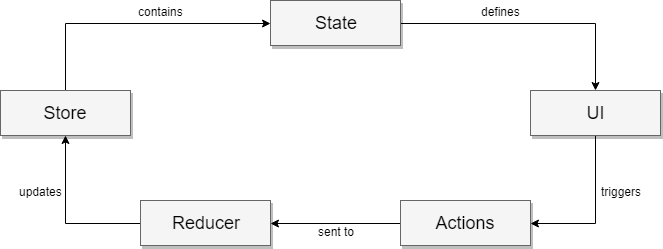
\includegraphics[width=1.0\textwidth]{img/reactReduxFlow.png}
\caption{React + Redux flow}
\label{fig04:reduxFlow}
\end{figure}

%%-----------------------------------------------------------------------------------------
\subsubsection{Communication With Other Modules}

To communicate with Fileserver module, we use axios library. It is a promise based HTTP client for the browser and node.js~\citep{axios}. We use it to send HTTP requests to Fileserver. It simplifies sending AJAX requests and provides modern Promise API. 
\par
WebSocket communication with Player module utilizes default WebSocket object that provides JavaScript. Upon establishing connection with Player, the created socket is stored in state. Actions that send messages to Player access this instance to do so. A callback function is provided to the constructor that handles incoming messages. Incoming messages are processed and corresponding action is triggered.
\par
Firebase provides software development kit~(SDK) in JavaScript for developers. Every communication with Database module utilizes this SDK. It provides methods to manipulate and read data as well as hook up callbacks. It is also used for user authentication.

\subsubsection{JavaScript Libraries Used}

We used multiple packages and libraries from Node.js Packet Manager~(NPM). We will mention important ones.
\par
Material-UI library offers styled React components in popular material design developed by Google. We used these components to create a modern and appealing UI which should look familiar to users.
\par
Reaxt-intl library is used to create a localized application. All strings in components are grouped in "messages.js" file next the files containing layout, marked with unique identifier and a default translation is supplied. When a string is needed its identifier is passed to a function from react-intl library which takes care of finding the right translation. When the application is built all strings are extracted to a JSON file. Multiple JSON files can be provided with different translations to support multiple languages.
\par
To execute AJAX requests we used Axios library. It simplifies creating these requests and provides modern Promise-based API.


%%-----------------------------------------------------------------------------------------
\subsection{Bringing The Module Together}

On module startup the browser is run and initialized. When it is ready the web application is loaded from local storage. The application is displayed and users can work with it. The web application utilizes message router provided by CEF to communicate with browser. We registered a callback function \texttt{cefQuery} in JavaScript that allows sending messages to browser code. After users log in local Fileserver and Player are started utilising \texttt{cefQuery} function and connected to. These can be shut down and users may connect to other modules from "Devices" menu. 
%%-----------------------------------------------------------------------------------------
%% SECTION
%%-----------------------------------------------------------------------------------------
\section{Database Module}

Database structure can be found in the documentation chapter\todo{link to documentation}. A few remarks on the
structure:
\begin{itemize}
    \item database design should allow to add new entity easily.
    \item user and establishment data are divided on public and private part. In firebase, access to high level node provides access to all child nodes. Everyone should be able to read public data, only owner should see the private data.
    \item to reduce data redundancy lists are used in libraries entity
    \item to get a new key for a new node, firebase default node key generator is used (push function)
    \item when a value is an id, it should always be stored as a string, even when the id is a number for more general use
\end{itemize}

\par
Besides data storage Firebase is used to provide user authentication. It offers options to authenticate by e-mail address and a few popular social network accounts. IDs generated by authentication service are used in database to identify users.